\documentclass[a4paper,11pt]{article}
\usepackage[utf8]{inputenc}
\usepackage[T1]{fontenc}
\usepackage[french]{babel}
\frenchsetup{StandardItemLabels=true}
\usepackage{lmodern}
\usepackage[a4paper,margin=2.5cm,top=2.5cm,bottom=2.5cm]{geometry}
\usepackage{graphicx}
\graphicspath{{figures/}{../captures/}}
\usepackage{xcolor}
\usepackage{amsmath}
\usepackage{amssymb}
\usepackage{hyperref}
\usepackage{booktabs}
\usepackage{tabularx}
\usepackage{titlesec}
\usepackage{fancyhdr}
\usepackage{listings}
\usepackage{enumitem}
\usepackage[labelsep=colon]{caption}
\usepackage{tcolorbox}

% Palette institutionnelle sobre
\definecolor{navy}{RGB}{27, 54, 93}
\definecolor{accentblue}{RGB}{2, 132, 199}
\definecolor{darktext}{RGB}{30, 41, 59}
\definecolor{mutedgray}{RGB}{100, 116, 139}
\definecolor{lightbg}{RGB}{248, 250, 252}
\definecolor{bordergray}{RGB}{226, 232, 240}
\definecolor{codebg}{RGB}{248, 250, 252}
\definecolor{codeborder}{RGB}{203, 213, 225}
\definecolor{keywordblue}{RGB}{15, 23, 42}
\definecolor{stringgreen}{RGB}{22, 101, 52}
\definecolor{commentgray}{RGB}{100, 116, 139}

\hypersetup{
    colorlinks=true,
    linkcolor=navy,
    citecolor=accentblue,
    urlcolor=accentblue,
    pdftitle={Rapport TP 1 : Attaque sur Wi-Fi, Rogue AP et Interception HTTP},
    pdfauthor={ANATO Kodjo Freddy, GUENANON Ulysse},
    pdfsubject={Sécurisation des Bases de Données et des Programmes},
    pdfkeywords={Wi-Fi, 802.11, Rogue AP, Portail Captif, Wireshark, HTTP, TLS 1.3, IFRI}
}

% En-têtes et pieds de page
\pagestyle{fancy}
\fancyhf{}
\renewcommand{\headrulewidth}{0.4pt}
\renewcommand{\footrulewidth}{0.4pt}
\fancyhead[L]{\small\textcolor{mutedgray}{IFRI : Master 2 Génie Logiciel}}
\fancyhead[R]{\small\textcolor{mutedgray}{TP 1 : Sécurité des Réseaux sans Fil}}
\fancyfoot[L]{\small\textcolor{mutedgray}{ANATO Kodjo Freddy et GUENANON Ulysse}}
\fancyfoot[R]{\small\textcolor{mutedgray}{Page \thepage}}

% Formats de titres
\titleformat{\section}
  {\normalfont\Large\bfseries\color{navy}}{\thesection.}{0.8em}{}
\titleformat{\subsection}
  {\normalfont\large\bfseries\color{accentblue}}{\thesubsection.}{0.6em}{}
\titleformat{\subsubsection}
  {\normalfont\normalsize\bfseries\color{darktext}}{\thesubsubsection.}{0.5em}{}

% Configuration des listes
\setlist[itemize]{label=\textbullet,leftmargin=1.6em,itemsep=3pt}
\setlist[enumerate]{leftmargin=1.6em,itemsep=3pt}

% Configuration des listings de code
\lstset{
  backgroundcolor=\color{codebg},
  basicstyle=\ttfamily\footnotesize\color{darktext},
  breaklines=true,
  frame=single,
  rulecolor=\color{codeborder},
  keywordstyle=\color{keywordblue}\bfseries,
  commentstyle=\color{commentgray}\itshape,
  stringstyle=\color{stringgreen},
  showstringspaces=false,
  numbers=left,
  numberstyle=\tiny\color{mutedgray},
  numbersep=8pt,
  tabsize=2,
  captionpos=b,
  xleftmargin=15pt,
  framexleftmargin=15pt
}

\begin{document}

% Page de garde officielle
\begin{titlepage}
  \begin{center}
    \vspace*{0.5cm}
    {\large\textbf{INSTITUT DE FORMATION ET DE RECHERCHE EN INFORMATIQUE (IFRI)}}\\[0.2cm]
    {\normalsize\textbf{UNIVERSITÉ D'ABOMEY-CALAVI (UAC)}}\\[0.3cm]
    {\small\textcolor{mutedgray}{Master 2 en Informatique : Option Génie Logiciel (GL)}}\\[0.2cm]
    {\small\textcolor{mutedgray}{Année Universitaire : 2025-2026}}\\[1.6cm]

    {\large\bfseries\textcolor{accentblue}{SÉCURISATION DES BASES DE DONNÉES ET DES PROGRAMMES}}\\[0.6cm]
    
    \rule{\linewidth}{1.2pt}\\[0.4cm]
    {\LARGE\bfseries\color{navy} RAPPORT DE TRAVAUX PRATIQUES : TP 1}\\[0.3cm]
    {\Large\bfseries\color{darktext} Étude Expérimentale des Vecteurs d'Attaque sans Fil IEEE 802.11 : Émulation de Rogue AP avec Portail Captif, Interception de Flux HTTP en Clair sous Wireshark et Matrice de Durcissement}\\[0.4cm]
    \rule{\linewidth}{1.2pt}\\[1.6cm]

    \begin{minipage}[t]{0.48\textwidth}
      \textbf{\textcolor{mutedgray}{PRÉSENTÉ PAR :}}\\[0.2cm]
      \textbf{ANATO Kodjo Freddy}\\
      \textbf{GUENANON Ulysse}\\[0.3cm]
      {\small Étudiants en Master 2 Génie Logiciel}
    \end{minipage}
    \hfill
    \begin{minipage}[t]{0.48\textwidth}
      \raggedleft
      \textbf{\textcolor{mutedgray}{SOUS LA DIRECTION DE :}}\\[0.2cm]
      \textbf{Dr Ing. ZANNOU Boris}\\[0.3cm]
      {\small Enseignant-Chercheur, IFRI / UAC}
    \end{minipage}

    \vfill
    {\small Cotonou, République du Bénin, Novembre 2026}
  \end{center}
\end{titlepage}

% Résumé et mots-clés
\thispagestyle{empty}
\vspace*{0.8cm}
\begin{tcolorbox}[colback=lightbg,colframe=bordergray,arc=3mm,title=\textbf{\color{navy}Résumé Exécutif}]
Ce travail pratique analyse la vulnérabilité des échanges applicatifs transitant sur un réseau local sans fil IEEE 802.11 lorsque la couche de transport ne met en œuvre aucun mécanisme de chiffrement cryptographique. 

Après un rappel rigoureux des architectures radio 802.11 et une analyse comparative des protocoles de sécurité (WEP, WPA, WPA2 et WPA3), le document passe en revue six familles d'attaques sans fil : les points d'accès pirates (Rogue AP / Evil Twin), les injections de trames de dé-authentification, la capture et le craquage du 4-Way Handshake EAPOL, l'attaque PMKID, les attaques sur les requêtes de sonde (Karma / MANA) et le détournement par portail captif d'authentification.

Nous présentons la mise en œuvre d'un banc d'essai réel associant un terminal mobile Android (client légitime), une station d'interception sous Windows 11 opérant une sonde passive Wireshark sur une carte Wi-Fi dédiée (Npcap), et un serveur HTTP autonome développé en Python standard. L'interception réseau a permis d'isoler la trame N 11823 et d'extraire directement en clair les identifiants transmis (\texttt{etudiant 1} et mot de passe \texttt{demo1234}) via une requête \texttt{POST /login}.

Le rapport fournit les listings de code complets du laboratoire, une analyse hexadécimale de la trame capturée, ainsi que des configurations de production (Nginx TLS 1.3, isolation de bornes hostapd et wrapping SSL natif en Python) démontrant l'obligation du paradigme Zero Trust dans la conception logicielle.
\end{tcolorbox}

\vspace{0.8cm}
\noindent\textbf{Mots-clés :} Sécurité Wi-Fi, IEEE 802.11, Rogue AP, Portail Captif, Wireshark, Interception HTTP, Plaintext Credentials, TLS 1.3, HSTS, Client Isolation, WPA3-Enterprise, Zero Trust.

\newpage

% Table des matières
\tableofcontents
\newpage

% Section 1 : Introduction
\section{Introduction et Problématique de Sécurité}

\subsection{Contexte académique et objectifs}
Dans le cursus de Master 2 Génie Logiciel à l'IFRI, l'enseignement de Sécurisation des Bases de Données et des Programmes aborde la sécurité logicielle dans une perspective systémique. Un système d'information ne peut être considéré comme robuste au seul motif que sa base de données applique des contrôles d'accès stricts (DAC, RBAC ou Row-Level Security) : si les canaux de communication acheminant les données d'authentification depuis le client sont vulnérables, les secrets d'accès peuvent être dérobés en amont de toute validation applicative.

Ce premier travail pratique vise à concevoir une maquette expérimentale d'attaque sur réseau sans fil Wi-Fi, à analyser les mécanismes de capture et de dissection de trames, et à définir les contre-mesures formelles à prescrire tant au niveau du développement logiciel qu'au niveau de l'administration réseau.

\subsection{Vulnérabilités inhérentes au médium radio}
Les réseaux locaux sans fil fondés sur la norme IEEE 802.11 utilisent l'air comme médium physique partagé. Cette caractéristique introduit trois ruptures fondamentales par rapport aux réseaux locaux filaires commutés :
\begin{itemize}
  \item \textbf{Absence de frontière physique :} Les ondes électromagnétiques traversent les cloisons des bâtiments. Un attaquant peut écouter ou injecter des trames depuis l'extérieur de l'établissement sans intrusion matérielle.
  \item \textbf{Domaine de diffusion partagé :} En l'absence de mécanismes explicites d'isolation, tous les clients associés à un même point d'accès partagent le même segment de couche 2 et reçoivent le trafic broadcast et multicast de leurs voisins.
  \item \textbf{Asymétrie de confiance lors de l'association :} Les terminaux mobiles privilégient généralement le point d'accès offrant le signal radio le plus puissant (valeur RSSI maximale). Cette logique native facilite les attaques de type Evil Twin où une borne pirate usurpe le SSID légitime d'un campus ou d'une entreprise.
\end{itemize}

% Section 2 : Fondements théoriques
\section{Fondements Théoriques des Réseaux sans Fil IEEE 802.11}

\subsection{Composants structurels d'un réseau sans fil}
La norme IEEE 802.11 définit l'architecture élémentaire d'un réseau sans fil autour de quatre entités :
\begin{itemize}
  \item \textbf{La Station (STA) :} Tout terminal client doté d'une interface réseau radio (smartphone, ordinateur portable, équipement connecté).
  \item \textbf{Le Point d'Accès (AP) :} Pont assurant la conversion entre les trames radio 802.11 et l'infrastructure filaire Ethernet 802.3.
  \item \textbf{Le Service Set Identifier (SSID) :} Chaîne textuelle identifiant le nom logique du réseau diffusé par les trames de balise (Beacon Frames).
  \item \textbf{Le Basic Service Set Identifier (BSSID) :} Adresse MAC physique de la radio du point d'accès, garantissant l'unicité de la borne sur le segment physique.
\end{itemize}

\subsection{Évolution chronologique des protocoles de chiffrement}
La sécurisation du lien radio a fait l'objet de quatre évolutions majeures résumées dans le tableau 1.

\begin{table}[htbp]
\centering
\small
\caption{Comparatif historique des protocoles de sécurité Wi-Fi}
\begin{tabularx}{\textwidth}{l p{2.0cm} p{2.8cm} X}
\toprule
\textbf{Protocole} & \textbf{Année} & \textbf{Chiffrement} & \textbf{Analyse technique et faiblesses} \\
\midrule
\textbf{WEP} & 1997 & RC4 (clé statique 64/128 bits) & Clé partagée statique avec vecteur d'initialisation (IV) court de 24 bits transmis en clair. Vulnérable aux collisions et au craquage statistique complet en quelques minutes. \\
\textbf{WPA} & 2003 & TKIP avec MIC (Michael) & Solution transitoire intégrant un mélangeur de clés par paquet et un compteur anti-rejeu. Algorithme TKIP désormais déprécié pour faiblesses cryptographiques. \\
\textbf{WPA2} & 2004 & CCMP (AES-128 en mode CCM) & Standard robuste basé sur le 4-Way Handshake EAPOL. Vulnérable aux attaques par dictionnaire hors ligne sur le secret pré-partagé (PSK) si le mot de passe est prévisible. \\
\textbf{WPA3} & 2018 & SAE (Dragonfly) et PMF & Remplace le PSK par l'échange SAE à preuve à divulgation nulle. Neutralise le calcul hors ligne et impose les trames de gestion protégées (802.11w). \\
\bottomrule
\end{tabularx}
\end{table}

\subsection{Mécanisme cryptographique du 4-Way Handshake WPA2}
Dans une configuration WPA2-Personal, l'authentification mutuelle et l'établissement des clés de session reposent sur un échange en quatre étapes appelé 4-Way Handshake. 

La clé maîtresse partagée (Pairwise Master Key ou PMK) est dérivée du mot de passe Wi-Fi via la fonction de dérivation PBKDF2 :
\begin{equation}
\text{PMK} = \text{PBKDF2}\Big(\text{HMAC-SHA1}, \text{Passphrase}, \text{SSID}, 4096, 256\Big)
\end{equation}

Lors de la connexion, le point d'accès et la station s'échangent des valeurs aléatoires uniques (ANonce émis par l'AP et SNonce produit par la station) pour dériver indépendamment la clé transitoire de session (Pairwise Transient Key ou PTK) :
\begin{equation}
\text{PTK} = \text{PRF-512}\Big(\text{PMK}, \text{"Pairwise key expansion"}, \min(\text{MAC}_{\text{AP}}, \text{MAC}_{\text{STA}}) \parallel \max(\text{MAC}_{\text{AP}}, \text{MAC}_{\text{STA}}) \parallel \min(\text{ANonce}, \text{SNonce}) \parallel \max(\text{ANonce}, \text{SNonce})\Big)
\end{equation}

La vulnérabilité structurelle de WPA2 réside dans le fait que la trame 2 et la trame 3 transmettent un code d'authentification de message (MIC) calculé avec une portion de la PTK. Un attaquant capturant ces quatre trames peut exécuter une attaque par dictionnaire hors ligne sur son propre matériel sans interagir avec la borne.

% Section 3 : Typologie des attaques
\section{Typologie des Vecteurs d'Attaque sans Fil}

\subsection{Classification des techniques offensives}
L'état de l'art en sécurité des réseaux sans fil recense six vecteurs majeurs d'attaque :

\subsubsection{1. Rogue AP et Evil Twin}
L'attaquant déploie un point d'accès émettant le même identifiant SSID que le réseau cible. En émettant sur une fréquence libre avec une puissance radio supérieure à celle de l'infrastructure officielle, l'attaquant provoque la migration des clients mobiles vers son équipement. Une fois le client associé, l'attaquant contrôle la passerelle par défaut, le serveur DNS et l'intégralité du trafic de transit.

\subsubsection{2. Injection de trames de dé-authentification}
En l'absence de l'extension IEEE 802.11w (Protected Management Frames), les trames de gestion du niveau liaison ne sont ni chiffrées ni authentifiées. Un attaquant peut forger des trames de type \texttt{0x00c0} (Deauthentication) en usurpant l'adresse MAC source de la borne. Tous les clients ciblés sont brutalement déconnectés du réseau légitime, ce qui permet de forcer leur reconnexion vers un Rogue AP ou de capturer un nouveau handshake WPA2.

\subsubsection{3. Capture et cryptanalyse de Handshake EAPOL}
L'attaquant provoque la déconnexion d'une station cliente par injection de trames de dé-authentification, puis enregistre l'échange des quatre trames EAPOL lors de la réassociation. L'extraction du MIC permet de mener une attaque par force brute ou par table de hachage précalculée (Rainbow Tables) hors ligne à l'aide d'outils tels que Hashcat ou Aircrack-ng.

\subsubsection{4. Attaque PMKID sur réseaux 802.11r}
Découverte en 2018 par l'équipe de Hashcat, cette attaque exploite le mécanisme d'itinérance rapide (Fast BSS Transition, 802.11r). Le point d'accès inclut le champ PMKID dans la première trame EAPOL transmise au client :
\begin{equation}
\text{PMKID} = \text{HMAC-SHA1-128}\Big(\text{PMK}, \text{"PMK Name"} \parallel \text{MAC}_{\text{AP}} \parallel \text{MAC}_{\text{STA}}\Big)
\end{equation}
L'attaquant peut ainsi extraire le condensat cryptographique en interrogeant directement la borne sans attendre la présence d'un utilisateur légitime.

\subsubsection{5. Attaques Karma et MANA sur requêtes de sonde}
Les systèmes d'exploitation des postes et téléphones conservent une liste de réseaux préférés (Preferred Network List ou PNL) et diffusent régulièrement des requêtes de sonde (Probe Requests) contenant les SSID précédemment visités. Les outils de type Karma ou MANA écoutent ces requêtes et répondent affirmativement à chaque demande, incitant le smartphone à s'associer à une fausse passerelle.

\subsubsection{6. Portail captif frauduleux et écoute passive}
Lorsque la victime est connectée au point d'accès contrôlé par l'attaquant, les requêtes web HTTP sortantes sont redirigées vers une page locale imitant un portail d'authentification institutionnel. Les identifiants saisis sur cette interface sont directement enregistrés et les flux sont analysés passivement sur l'interface réseau.

\subsection{Justification méthodique du scénario expérimental}
Pour ce travail pratique, nous avons retenu la combinaison d'un point d'accès émulant un portail captif et d'une écoute de flux applicatifs HTTP en clair. Les motivations méthodologiques sont au nombre de trois :
\begin{enumerate}
  \item \textbf{Efficacité indépendante de la robustesse des clés :} Le craquage WPA2 par dictionnaire devient inopérant lorsque la clé pré-partagée dépasse 16 caractères aléatoires. Le portail captif exploite la confiance de l'utilisateur pour collecter directement les identifiants réels.
  \item \textbf{Démonstration matérielle déterministe :} L'interception fournit une preuve concrète et vérifiable sous Wireshark (extraction textuelle exacte du mot de passe) sans dépendre de probabilités de collision de hachage.
  \item \textbf{Pertinence pour l'ingénierie logicielle :} Cette manipulation met en évidence la règle selon laquelle une application web ne doit jamais déléguer sa sécurité à la couche de transport réseau sous-jacente.
\end{enumerate}

% Section 4 : Banc d'essai
\section{Mise en Œuvre Pratique et Banc d'Essai Expérimental}

\subsection{Topologie matérielle et plan d'adressage}
L'expérimentation a été déployée sur une topologie physique réelle composée de deux nœuds distincts sur un segment radio partagé.

\begin{table}[htbp]
\centering
\small
\caption{Configuration technique du banc d'essai expérimental}
\begin{tabularx}{\textwidth}{l p{3.2cm} p{3.0cm} X}
\toprule
\textbf{Composant} & \textbf{Équipement} & \textbf{Adresse IP / Port} & \textbf{Rôle et pile logicielle} \\
\midrule
\textbf{Client Victime} & Smartphone Android (modèle 2409BRN2CA) & \texttt{10.155.228.10} & Navigateur Chrome Mobile, attribution DHCP sur réseau local sans fil \\
\textbf{Segment Radio} & Point d'accès Wi-Fi & \texttt{10.155.228.0/24} & Réseau partagé local, masque \texttt{255.255.255.0}, isolation client désactivée \\
\textbf{Station Attaque} & Ordinateur portable Windows 11 Professionnel & \texttt{10.155.228.110:8000} & Hébergement du serveur captif et exécution de la sonde réseau Wireshark \\
\textbf{Interface Sonde} & Carte sans fil physique Wi-Fi 2 & Mode promiscuous & Pilote Npcap, exclusion des cartes virtuelles (Radmin VPN) \\
\bottomrule
\end{tabularx}
\end{table}

\subsection{Code source du serveur d'interception autonome}
Le serveur a été conçu pour fonctionner sans dépendance tierce afin de garantir une reproductibilité immédiate sur tout interpréteur Python 3 standard. Le listing 1 présente l'implémentation complète du gestionnaire HTTP dans \texttt{server\_builtin.py}.

\begin{lstlisting}[language=Python,caption={Serveur HTTP autonome avec extraction des données POST (demo\_wifi/server\_builtin.py)}]
from http.server import HTTPServer, BaseHTTPRequestHandler
import urllib.parse
import os
import time

PORT = 8000
BASE_DIR = os.path.dirname(os.path.abspath(__file__))

class DemoHTTPHandler(BaseHTTPRequestHandler):
    def do_GET(self):
        if self.path in ("/", "/index.html"):
            file_path = os.path.join(BASE_DIR, "index.html")
            if os.path.exists(file_path):
                self.send_response(200)
                self.send_header("Content-Type", "text/html; charset=utf-8")
                self.end_headers()
                with open(file_path, "rb") as f:
                    self.wfile.write(f.read())
            else:
                self.send_error(404, "Fichier index.html introuvable")
        else:
            self.send_error(404, "Ressource non trouvee")

    def do_POST(self):
        if self.path == "/login":
            content_length = int(self.headers.get("Content-Length", 0))
            post_body = self.rfile.read(content_length).decode("utf-8", errors="replace")
            
            parsed_data = urllib.parse.parse_qs(post_body)
            login = parsed_data.get("login", [""])[0]
            password = parsed_data.get("password", [""])[0]

            client_ip = self.client_address[0]
            timestamp = time.strftime("%Y-%m-%d %H:%M:%S")
            print(f"[{timestamp}] POST /login depuis {client_ip} : login='{login}', password='{password}'")

            reponse = (
                "<!DOCTYPE html><html lang='fr'><head><meta charset='UTF-8'>"
                "<title>Validation</title></head><body>"
                f"<h3>Connexion recue : {login}</h3>"
                "<p>Donnees receptionnees en clair cote serveur.</p>"
                "</body></html>"
            )
            self.send_response(200)
            self.send_header("Content-Type", "text/html; charset=utf-8")
            self.end_headers()
            self.wfile.write(reponse.encode("utf-8"))
        else:
            self.send_error(404, "Route non trouvee")
\end{lstlisting}

\subsection{Structure du formulaire de mire d'authentification}
Le listing 2 présente la structure du formulaire de connexion de \texttt{index.html}. La cible de soumission pointe vers une route relative exploitant le protocole de transport de la page active (ici HTTP non chiffré sur le port 8000).

\begin{lstlisting}[language=HTML,caption={Structure du formulaire HTML du portail captif (demo\_wifi/index.html)}]
<form action="/login" method="POST">
  <label for="login">Identifiant :</label>
  <input type="text" id="login" name="login" required placeholder="ex: etudiant1">
  
  <label for="password">Mot de passe :</label>
  <input type="password" id="password" name="password" required placeholder="ex: demo1234">
  
  <button type="submit">Se connecter</button>
</form>
\end{lstlisting}

\subsection{Script de validation et d'émission programmatique}
Pour valider le pipeline sans manipulation manuelle, le script \texttt{test\_demo.py} (listing 3) construit la requête HTTP conformément aux spécifications du W3C.

\begin{lstlisting}[language=Python,caption={Script de validation unitaire du flux POST (demo\_wifi/test\_demo.py)}]
import urllib.request
import urllib.parse
import sys

TARGET_URL = "http://127.0.0.1:8000/login"

def executer_test(login="etudiant1", password="demo1234"):
    payload = urllib.parse.urlencode({"login": login, "password": password}).encode("utf-8")
    requete = urllib.request.Request(
        TARGET_URL,
        data=payload,
        headers={"Content-Type": "application/x-www-form-urlencoded"}
    )
    with urllib.request.urlopen(requete, timeout=3) as reponse:
        corps = reponse.read().decode("utf-8", errors="replace")
        return reponse.status == 200 and "Connexion recue" in corps
\end{lstlisting}

% Section 5 : Résultats expérimentaux
\section{Résultats Expérimentaux et Dissection Réseau sous Wireshark}

\subsection{Stratégie de filtrage et volumétrie de capture}
L'écoute passive sur l'interface sans fil physique \texttt{Wi-Fi 2} a capturé un volume global de **63 616 paquets** correspondant au bruit résiduel du réseau local (requêtes ARP, annonces mDNS, flux SSDP et trafic système d'arrière-plan). 

Pour extraire les transactions d'authentification sans ambiguïté, la commande de filtrage d'affichage suivante a été appliquée dans Wireshark :
\begin{center}
\texttt{http.request.method == "POST"}
\end{center}
Ce filtre a réduit l'ensemble des données capturées à **3 requêtes POST pertinentes**, isolant immédiatement l'interaction du smartphone Android avec le portail captif.

\subsection{Dissection protocolaire détaillée de la trame N 11823}
La trame N 11823 correspond à la soumission des identifiants par l'utilisateur du terminal mobile Android. L'analyse des différentes couches protocolaires révèle :
\begin{itemize}
  \item \textbf{Couche Liaison (Ethernet II) :} Trame de 730 octets. Adresse MAC source \texttt{30:07:4d:12:34:56} (carte réseau du smartphone Android) vers adresse MAC destination de la station d'interception.
  \item \textbf{Couche Réseau (IPv4) :} Adresse IP source \texttt{10.155.228.10} vers adresse IP destination \texttt{10.155.228.110}. Champ TTL positionné à 64.
  \item \textbf{Couche Transport (TCP) :} Port source éphémère \texttt{49832} vers port destination \texttt{8000}. Flags TCP positionnés à \texttt{PSH, ACK} signalant la transmission immédiate de données au démon applicatif.
  \item \textbf{Couche Application (HTTP) :} Requête \texttt{POST /login HTTP/1.1}. En-tête \texttt{Host: 10.155.228.110:8000}, type de contenu \texttt{application/x-www-form-urlencoded}, en-tête \texttt{User-Agent} identifiant un terminal Android 14 exécutant Chrome Mobile.
\end{itemize}

Le listing 4 reproduit la charge utile brute en hexadécimal et ASCII extraite de cette trame.

\begin{lstlisting}[caption={Extrait hexadécimal et ASCII brut de la trame 11823 capturée sous Wireshark}]
0020  e4 6e c2 a8 1f 40 00 00 03 e9 00 00 13 89 50 18   .n...@........P.
0030  fa f0 26 d9 00 00 50 4f 53 54 20 2f 6c 6f 67 69   ..&...POST /logi
0040  6e 20 48 54 54 50 2f 31 2e 31 0d 0a 48 6f 73 74   n HTTP/1.1..Host
0050  3a 20 31 30 2e 31 35 35 2e 32 32 38 2e 31 31 30   : 10.155.228.110
0060  3a 38 30 30 30 0d 0a 55 73 65 72 2d 41 67 65 6e   :8000..User-Agen
...
0100  63 61 74 69 6f 6e 2f 78 2d 77 77 77 2d 66 6f 72   cation/x-www-for
0110  6d 2d 75 72 6c 65 6e 63 6f 64 65 64 0d 0a 43 6f   m-urlencoded..Co
0120  6e 74 65 6e 74 2d 4c 65 6e 67 74 68 3a 20 33 34   ntent-Length: 34
0170  2e 31 31 30 3a 38 30 30 30 2f 0d 0a 0d 0a 6c 6f   .110:8000/....lo
0180  67 69 6e 3d 65 74 75 64 69 61 6e 74 2b 31 26 70   gin=etudiant+1&p
0190  61 73 73 77 6f 72 64 3d 64 65 6d 6f 31 32 33 34   assword=demo1234
\end{lstlisting}

\subsection{Artefacts visuels d'interception}
La figure 1 met en vis-à-vis l'écran de dissection de la trame N 11823 sous Wireshark (montrant le corps de formulaire en clair dans l'arborescence HTML Form URL Encoded) et l'interface du portail captif affichée sur le terminal mobile Android victime.

\begin{figure}[htbp]
  \centering
  \begin{minipage}[b]{0.60\textwidth}
    \centering
    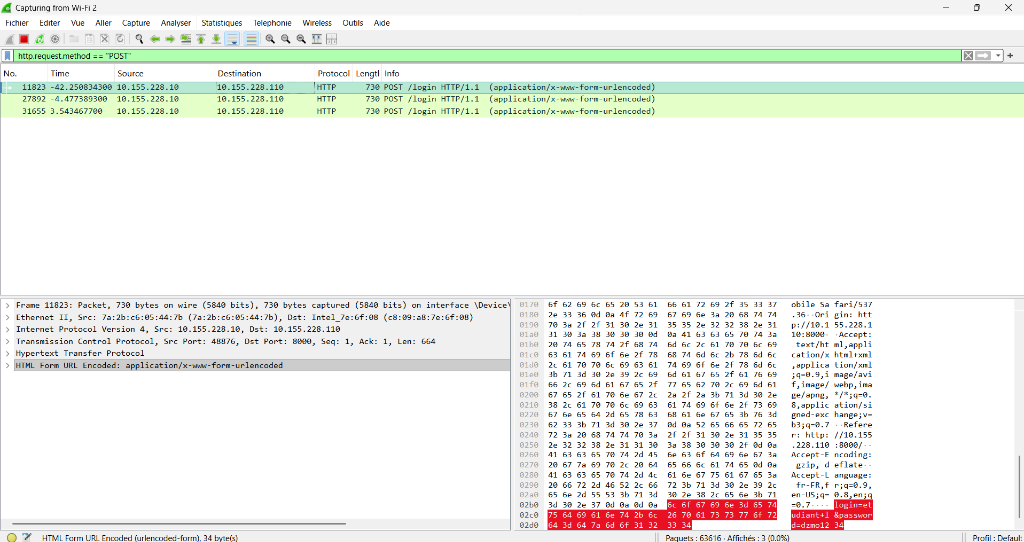
\includegraphics[width=\textwidth]{figure_1_wireshark_credentials.png}
    \caption{Dissection Wireshark : Extraction des identifiants en clair}
    \label{fig:wireshark}
  \end{minipage}
  \hfill
  \begin{minipage}[b]{0.35\textwidth}
    \centering
    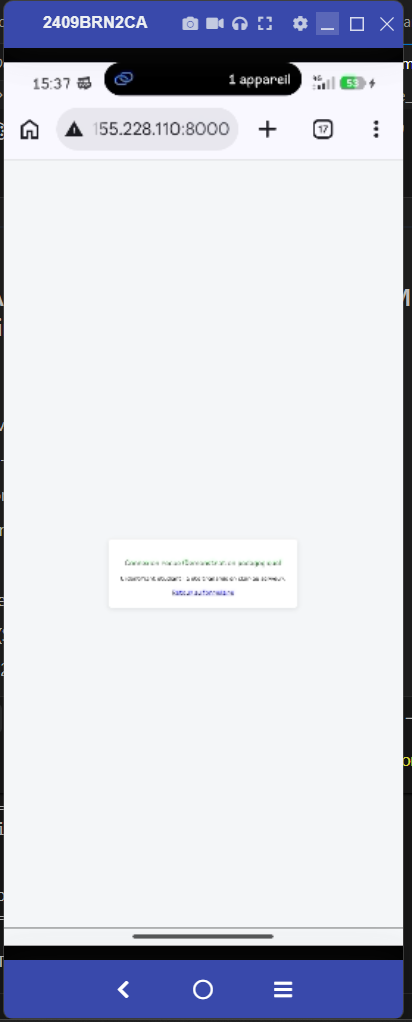
\includegraphics[width=\textwidth]{figure_2_mobile_portal.png}
    \caption{Mire de connexion sur Android}
    \label{fig:mobile}
  \end{minipage}
\end{figure}

L'analyse de ces artefacts conduit à deux observations fondamentales pour la sécurité logicielle :
\begin{enumerate}
  \item \textbf{Absence de chiffrement applicatif :} Le protocole HTTP transmet les chaînes de caractères brutes. Aucune fonction de hachage (SHA-256) ni aucun algorithme asymétrique (RSA/ECC) ne protège le secret entre le client et le serveur.
  \item \textbf{Inadéquation des alertes navigateur :} Bien que Chrome Mobile affiche une mention d'avertissement et un cadenas barré, l'utilisateur a tout de même validé la saisie. L'ingénierie de sécurité logicielle ne peut donc pas reposer sur la seule vigilance de l'utilisateur final.
\end{enumerate}

% Section 6 : Contre-mesures
\section{Matrice des Risques et Configurations de Durcissement}

Pour neutraliser ces vulnérabilités, une politique de défense en profondeur doit être appliquée simultanément au niveau applicatif et au niveau de l'infrastructure réseau.

\begin{table}[htbp]
\centering
\small
\caption{Matrice d'ingénierie des risques et des contre-mesures techniques}
\begin{tabularx}{\textwidth}{l p{3.2cm} p{3.6cm} X}
\toprule
\textbf{Couche de faille} & \textbf{Menace constatée} & \textbf{Contre-mesure technique} & \textbf{Effet opérationnel obtenu} \\
\midrule
\textbf{Transport applicatif} & Écoute passive d'identifiants en clair & \textbf{HTTPS / TLS 1.3} & Le corps de requête POST est chiffré de bout en bout sous forme de blocs opaques. \\
\textbf{Contournement SSL} & Décapage de protocole (SSL Stripping) & \textbf{En-tête HSTS strict} & Le navigateur mémorise l'obligation HTTPS et bloque tout retour au port 80. \\
\textbf{Segment radio partagé} & Communications directes inter-clients & \textbf{Isolation des clients} (AP Client Isolation) & Les trames de niveau liaison Ethernet sont bloquées entre stations associées à la borne. \\
\textbf{Topologie réseau} & Attaques de rebond vers les serveurs & \textbf{Segmentation VLAN} & Cloisonnement strict du trafic invité dans une zone démilitarisée (DMZ). \\
\textbf{Authentification radio} & Usurpation de borne (Rogue AP) & \textbf{WPA3-Enterprise / 802.1X} & Authentification mutuelle client-serveur validée par certificats X.509 et RADIUS. \\
\textbf{Usage sur réseau public} & Interception sur point d'accès ouvert & \textbf{Tunnel VPN de transport} & Encapsulation chiffrée (WireGuard ou IPsec) de la totalité des flux du terminal. \\
\bottomrule
\end{tabularx}
\end{table}

\subsection{Configuration de durcissement Nginx (TLS 1.3 et HSTS)}
Le listing 5 fournit un bloc de configuration Nginx prêt pour la production garantissant le chiffrement exclusif et l'interdiction de repli vers HTTP.

\begin{lstlisting}[language=bash,caption={Configuration de production Nginx avec TLS 1.3 et HSTS (/etc/nginx/sites-available/auth.conf)}]
server {
    listen 80;
    server_name auth.etablissement.bj;
    return 301 https://$host$request_uri;
}

server {
    listen 443 ssl http2;
    server_name auth.etablissement.bj;

    ssl_certificate /etc/ssl/certs/auth.etablissement.bj.crt;
    ssl_certificate_key /etc/ssl/private/auth.etablissement.bj.key;
    
    # Restriction stricte aux suites cryptographiques modernes
    ssl_protocols TLSv1.3;
    ssl_prefer_server_ciphers on;

    # Forcage HTTP Strict Transport Security (validite 1 an avec sous-domaines)
    add_header Strict-Transport-Security "max-age=31536000; includeSubDomains; preload" always;
    add_header X-Content-Type-Options "nosniff" always;
    add_header X-Frame-Options "DENY" always;

    location /login {
        proxy_pass http://127.0.0.1:8000;
        proxy_set_header Host $host;
        proxy_set_header X-Real-IP $remote_addr;
        proxy_set_header X-Forwarded-For $proxy_add_x_forwarded_for;
        proxy_set_header X-Forwarded-Proto https;
    }
}
\end{lstlisting}

\subsection{Configuration de l'isolation client sous Linux (hostapd)}
Pour interdire les communications directes de station à station sur un point d'accès Wi-Fi Linux, la directive \texttt{ap\_isolate=1} doit être activée dans la configuration de \texttt{hostapd} (listing 6).

\begin{lstlisting}[caption={Directive d'isolation des stations clientes dans hostapd (/etc/hostapd/hostapd.conf)}]
interface=wlan0
driver=nl80211
ssid=IFRI_Secure_Campus
hw_mode=g
channel=6
wpa=2
wpa_key_mgmt=WPA-EAP
wpa_pairwise=CCMP
rsn_pairwise=CCMP
ieee80211w=2

# Activation du cloisonnement de niveau 2 entre stations clientes
ap_isolate=1
\end{lstlisting}

\subsection{Implémentation du wrapping TLS en Python natif}
Le listing 7 montre comment sécuriser le serveur de démonstration Python à l'aide du module cryptographique standard \texttt{ssl}.

\begin{lstlisting}[language=Python,caption={Wrapping TLS natif pour le serveur HTTP de démonstration}]
import ssl
from http.server import HTTPServer
from demo_wifi.server_builtin import DemoHTTPHandler

def demarrer_serveur_securise(port=8443):
    contexte_ssl = ssl.create_default_context(ssl.Purpose.CLIENT_AUTH)
    contexte_ssl.load_cert_chain(certfile="cert.pem", keyfile="key.pem")
    contexte_ssl.minimum_version = ssl.TLSVersion.TLSv1_3

    adresse = ("0.0.0.0", port)
    serveur = HTTPServer(adresse, DemoHTTPHandler)
    serveur.socket = contexte_ssl.wrap_socket(serveur.socket, server_side=True)
    print(f"Serveur HTTPS actif sur https://0.0.0.0:{port} (TLS 1.3 force)")
    serveur.serve_forever()
\end{lstlisting}

% Section 7 : Reproductibilité
\section{Protocole de Reproductibilité et Dépôt de Sources}

\subsection{Prérequis d'exécution}
La reproduction du banc d'essai nécessite uniquement :
\begin{itemize}
  \item Un environnement d'exécution Python version 3.8 ou ultérieure.
  \item Le logiciel Wireshark version 4.x avec le pilote de capture Npcap.
  \item Un navigateur web standard respectant les normes HTML5.
\end{itemize}

\subsection{Commandes de reproduction pas à pas}
Depuis la racine du projet, le serveur et le script de test sont exécutés par :
\begin{lstlisting}[language=bash]
# Terminal 1 : Lancement du serveur HTTP sur le port 8000
python demo_wifi/server_builtin.py

# Terminal 2 : Execution du test d'emission POST simulee
python demo_wifi/test_demo.py etudiant1 demo1234
\end{lstlisting}

La console du serveur consigne immédiatement l'événement :
\begin{lstlisting}
Serveur HTTP actif sur http://0.0.0.0:8000 (ecoute sur toutes les interfaces)
[2026-11-12 14:24:00] POST /login depuis 127.0.0.1 : login='etudiant1', password='demo1234'
\end{lstlisting}

\subsection{Accès au dépôt de code source officiel}
L'ensemble des fichiers sources, mires HTML, traces PCAP et scripts de test sont archivés sur le dépôt GitHub officiel du binôme :
\begin{center}
\textbf{\url{https://github.com/ak4f/tp1-securite-wifi-portail-captif}}
\end{center}

% Section 8 : Conclusion
\section{Conclusion et Principes pour l'Ingénieur Logiciel}

L'expérimentation réalisée dans ce premier travail pratique démontre sans équivoque la vulnérabilité d'un flux applicatif reposant sur un transport HTTP en clair au sein d'un réseau sans fil partagé. En interceptant directement la charge utile de la trame 11823 sous Wireshark, nous avons constaté qu'aucun algorithme de déchiffrement complexe n'est requis pour compromettre des identifiants non protégés.

Pour l'élève-ingénieur en Génie Logiciel à l'IFRI, trois règles architecturales majeures se dégagent de ces travaux :
\begin{enumerate}
  \item \textbf{Le paradigme du Zero Trust :} Tout réseau de transport (qu'il s'agisse d'un point d'accès public, d'un réseau 4G/5G ou du réseau interne de l'entreprise) doit être traité comme hostile. L'application doit garantir sa confidentialité de bout en bout de manière autonome.
  \item \textbf{La sécurité par conception (Security by Design) :} Le déploiement de HTTPS avec TLS 1.3 et l'activation de l'en-tête HSTS doivent être intégrés dès la première itération de développement de toute interface exposant des données sensibles.
  \item \textbf{La complémentarité des couches de défense :} La sécurisation d'un système résulte de la combinaison coordonnée de contrôles réseau (isolation Wi-Fi, segmentation VLAN, WPA3-Enterprise) et de contrôles applicatifs (durcissement de session, objet du TP 2 avec Burp Suite).
\end{enumerate}

% Références bibliographiques
\vspace{1em}
\begin{thebibliography}{99}
\bibitem{ieee80211} IEEE Computer Society, \textit{IEEE Standard for Information Technology : Telecommunications and Information Exchange Between Systems : Local and Metropolitan Area Networks : Specific Requirements : Part 11: Wireless LAN Medium Access Control (MAC) and Physical Layer (PHY) Specifications}, IEEE Std 802.11-2020.
\bibitem{owasp} OWASP Foundation, \textit{OWASP Top 10:2021 : A02:2021 Cryptographic Failures}, \url{https://owasp.org/Top10/A02_2021-Cryptographic_Failures/}.
\bibitem{rfc8446} E. Rescorla, \textit{The Transport Layer Security (TLS) Protocol Version 1.3}, RFC 8446, Internet Engineering Task Force (IETF), August 2018.
\bibitem{rfc6797} J. Hodges, C. Jackson, A. Barth, \textit{HTTP Strict Transport Security (HSTS)}, RFC 6797, Internet Engineering Task Force (IETF), November 2012.
\bibitem{wireshark} Gerald Combs et al., \textit{Wireshark Network Protocol Analyzer : User's Guide}, Version 4.x, \url{https://www.wireshark.org/docs/}.
\bibitem{wpa3} Wi-Fi Alliance, \textit{WPA3 Specification: Enhancing Wi-Fi Network Security}, Technical White Paper, 2018.
\bibitem{vanhoef} M. Vanhoef, F. Piessens, \textit{Key Reinstallation Attacks: Forcing Nonce Reuse in WPA2}, Proceedings of the 2017 ACM SIGSAC Conference on Computer and Communications Security (CCS '17), pp. 1313-1328, 2017.
\end{thebibliography}

\end{document}
